\section{Periods with at most five pieces}\label{sec:terminal}

By \cref{thm:at-most-five}, a competitive normal vertex period whose state stays in the compact
domain has at most five pieces. This section computes the cost of every normal vertex period with
at most five pieces and shows that it is at least $\Aoct$, with equality only for the octagon's
trajectory. It then completes the proofs of \cref{thm:control} and of part~(b) of
\cref{thm:main}.

For so few pieces nothing has to be estimated abstractly. The tangent closure
(\cref{lem:tangent-closure}) is a system of four scalar equations in the factors; with at most
five factors it either has no solution or determines the factors up to one or two parameters.
The twist $X(T)=R^{-1}X(0)R$ then determines the initial state, and the cost becomes an explicit
function of the parameters. The difficulty is that the comparison is sharp. The four-piece
family contains the octagon, so its minimum must be located exactly, and the five-piece family
approaches the octagon at the edge of its domain, where one of its factors tends to~$1$ and the
period degenerates into the octagon's four pieces. Its strict inequality therefore has no margin
near that edge.

\subsection{Closed vertex cycles}\label{sec:terminal-cycles}

The terminal comparison uses only the data of a period at its switches. We write them in the
triangular coordinates $M\mapsto CMC^{-1}$,
$C=\begin{psmallmatrix}\sqrt3&1\\\sqrt3&-1\end{psmallmatrix}$, in which the tangent factors of
\cref{lem:one-arc} and the rotation $R$ become
\begin{equation}\label{eq:term-tri}
\begin{gathered}
 \widetilde T_0(q)=\begin{pmatrix}q&0\\0&q^{-1}\end{pmatrix},\qquad
 \widetilde T_1(q)=\begin{pmatrix}q^{-1}&q-q^{-1}\\0&q\end{pmatrix},\\
 \widetilde T_2(q)=\begin{pmatrix}q^{-1}&0\\q^{-1}-q&q\end{pmatrix},\qquad
 \widetilde R=\begin{pmatrix}0&1\\-1&1\end{pmatrix}
\end{gathered}
\end{equation}

\begin{definition}[Closed vertex cycle]\label{def:term-cycle}
A \emph{closed vertex cycle} with $N\ge1$ pieces consists of labels $i_k\in\Z/3$, factors $q_k>1$
and switch margins $m_k=(m_k(0),m_k(1),m_k(2))$ with positive entries, indexed by $k\in\Z$,
such that for every $k$ and $j$:
\begin{enumerate}
\item (twist) $i_{k+N}=i_k+1$, $q_{k+N}=q_k$, $m_{k+N}(j)=m_k(j-1)$, and $i_{k+1}\ne i_k$;
\item (quadric) $m_k(0)m_k(1)+m_k(1)m_k(2)+m_k(2)m_k(0)=4$;
\item (one-arc map) with $i=i_k$, $a=m_k(i)$, $b=m_k(i+1)$, $c=m_k(i-1)$,
 \begin{equation}\label{eq:term-arc}
  m_{k+1}(i)=a,\qquad m_{k+1}(i+1)=(a+b)q_k-a,\qquad m_{k+1}(i-1)=\frac{a+c}{q_k}-a;
 \end{equation}
\item (tangent closure)
 $\widetilde T_{i_k}(q_k)\,\widetilde T_{i_{k+1}}(q_{k+1})\cdots\widetilde T_{i_{k+N-1}}(q_{k+N-1})=\widetilde R$.
\end{enumerate}
Its \emph{raw cost} is $\sum_{k=0}^{N-1}\rho(a_k,b_k,c_k,q_k)$, where $a_k,b_k,c_k$ are the
active, growing and decreasing margins of item~(3) and
\begin{equation}\label{eq:term-rawarc}
 \rho(a,b,c,q)=a\bigl((a+b)(q-1)+(a+c)(1-q^{-1})-a\log q\bigr).
\end{equation}
\end{definition}

The letter $\rho$ denotes the raw arc cost only in this section and in
\cref{app:terminal-estimates}.

\begin{lemma}[The cycle of a normal period]\label{lem:term-cycle}
Let $P$ be a normal vertex period with $N$ pieces. Its labels, its factors and the margins
$m_k(j)=p_j$ of its twisted state at the switching times $\tau_k$ form a closed vertex cycle with
$N$ pieces, and
\[
 \cost(P)=\frac{\sqrt3}{4}\,\bigl(\text{raw cost}\bigr),\qquad\text{that is,}\qquad
 \frac{\cost(P)}{\sqrt{12}}=\frac{\text{raw cost}}{8}.
\]
\end{lemma}

\begin{proof}
Positivity and the quadric are \cref{lem:margins}; \eqref{eq:term-arc} and the cost of a piece,
$(\sqrt3/4)\,\rho(a,b,c,q)$, are \cref{lem:one-arc}. The twist $Y(t+T)=R^{-1}Y(t)R$ of the state
shifts the margins, $p_j(R^{-1}XR)=p_{j-1}(X)$, which gives $m_{k+N}(j)=m_k(j-1)$. The tangent
closure from the switch $\tau_k$ is \cref{lem:tangent-closure} for the period rebased at
$\tau_k$, conjugated by $C$.
\end{proof}

So a period beats the octagon exactly when the raw cost of its cycle is below $8\doct$.
Two operations change a cycle without changing its raw cost: \emph{rebasing}, which shifts all
indices by a fixed integer, and \emph{relabeling}, which adds $1$ to every label and shifts the
margins accordingly; rebasing a cycle with $N$ pieces by $r$ replaces its word by the last
$N-r$ letters followed by the first $r$ letters increased by one. Relabeling at most twice makes
the first label~$0$.

\subsection{The words of at most five pieces}\label{sec:terminal-words}

A cycle with first label $0$ is described by its word $i_0i_1\cdots i_{N-1}$: neighbouring
letters differ, and by the twist the letter after $i_{N-1}$ is $i_0+1=1$, so $i_{N-1}\ne1$.
For $N\le5$ there are $1+1+3+5+11=21$ such words.

\begin{proposition}[Words of at most five pieces]\label{prop:terminal-words}
Let $c$ be a closed vertex cycle with $N\le5$ pieces.
\begin{enumerate}
\item $N\ge4$.
\item If $N=4$, every switch is forward: $i_{k+1}=i_k+1$ for all $k$.
\item If $N=5$, either every switch is reverse, or some rebasing and relabeling of $c$ has the
 word $0\,1\,0\,2\,0$ and the same raw cost.
\end{enumerate}
\end{proposition}

\begin{proof}
Relabel so that $i_0=0$ and compare the closure product of each of the $21$ words with
$\widetilde R$, entry by entry. Each entry of a product of the matrices~\eqref{eq:term-tri} is
a rational function of the factors, and for most words a single entry already contradicts
$q_k>1$. For the word $0$, the upper left entry of $\widetilde T_0(q_0)$ is $q_0\neq0$. For
$02$, $020$, $0202$ and $02020$ the upper right entry of the product vanishes, while that of
$\widetilde R$ is~$1$; for $010$ and $01010$ the lower left entry vanishes instead of being
$-1$; for $0210$ and $02010$ the upper left entry is a positive monomial in the factors instead
of~$0$. For $012$ two entries are needed: the lower row of the product is
\[
 \Bigl(-\frac{q_1(q_2^2-1)}{q_0q_2},\ \frac{q_1q_2}{q_0}\Bigr),
\]
whose second entry forces $q_0=q_1q_2$, after which the first is $-(q_2^2-1)/q_2^2\ne-1$. The
words $0102$, $01012$ and $01212$ fall in the same way, through the two entries of the lower row:
for $01212$, the lower right entry gives $q_0q_2q_3=q_1q_4(q_2^2+q_3^2-1)$, and then the lower left
entry is $-1+q_1q_3/(q_0q_2q_4)\ne-1$. For $0212$, the upper left and lower left entries give
$q_2^2q_3^2=q_2^2+q_3^2$ and $q_0q_2=q_1q_3$, and then the lower right entry forces $q_2=1$. \Cref{tab:terminal-words} lists the outcome. The surviving words are
$0120$, whose switches, including the one across the seam to the letter $1$, are all forward;
the five words $01020$, $01202$, $01210$, $02012$, $02120$, which are the rebasings of $01020$,
normalized to start with~$0$; and $02102$, whose five switches are all reverse.
\end{proof}

\begin{table}[htbp]
\centering
\begin{tabular}{@{}l>{\raggedright\arraybackslash}p{0.42\textwidth}l@{}}
\toprule
$N$ & words with $i_0=0$, $i_{N-1}\ne1$ & outcome\\
\midrule
$1,2,3$ & $0$; $02$; $010$, $012$, $020$ & excluded by the closure\\
$4$ & $0102$, $0202$, $0210$, $0212$ & excluded by the closure\\
    & $0120$ \ ($++++$) & the octagon's word\\
$5$ & $01010$, $01012$, $01212$, $02010$, $02020$ & excluded by the closure\\
    & $01020$ \ ($+--++$), $01202$, $01210$, $02012$, $02120$ & rebasings of $01020$\\
    & $02102$ \ ($-----$) & entirely reverse (class $\cls{R}$)\\
\bottomrule
\end{tabular}
\caption{The reduced words of at most five letters and their fate. The signs are those of the
$N$ switches of a period, the last one across the seam.}
\label{tab:terminal-words}
\end{table}

\begin{remark}\label{rem:terminal-words-route}
Most of these words can also be excluded by the fixed-edge obstruction \cite{Notes}: a trajectory
whose control has one coordinate equal to zero almost everywhere cannot satisfy $g(T)=R$. On a
fixed edge of the control simplex the frame can be integrated explicitly, and the terminal
condition then forces $x(0)=-1/\sqrt3$, on the boundary of the star domain. Rebasing a word that
misses a letter in a suitable window produces such a trajectory. The entries of the closure give
the same exclusions without integrating along an edge, and neither argument uses optimality.
\end{remark}

\subsection{Four pieces}\label{sec:terminal-four}

By \cref{prop:terminal-words} and a relabeling, a four-piece cycle has the octagon's word
$2\,0\,1\,2$. Its closure equations can be solved in closed form.

\begin{lemma}[Four-piece closure]\label{lem:four-closure}
If $p,q,r,z>1$ and
\[\widetilde T_2(p)\widetilde T_0(q)\widetilde T_1(r)\widetilde T_2(z)=\widetilde R,\]
then $r=p$,
$z=q$ and $p^2q^2=p^2+q^2$.
\end{lemma}

\begin{proof}
The upper row of the product is
$\bigl(-q(r^2z^2-r^2-z^2)/(prz),\ qz(r^2-1)/(pr)\bigr)$, so $r^2z^2=r^2+z^2$ and
$qz(r^2-1)=pr$; together these give $pz=qr$. The lower right entry then gives
$q^2r^2=q^2+r^2$. Subtracting the two quadratic relations gives $(q^2-z^2)(r^2-1)=0$, so $z=q$,
and $pz=qr$ gives $r=p$.
\end{proof}

Write $a=1/p$ and $b=1/q$. The relation $p^2q^2=p^2+q^2$ becomes $a^2+b^2=1$: the four factors
are $(1/a,1/b,1/a,1/b)$ for a point $(a,b)$ of the open quarter circle, and every such point
satisfies the closure. Put
\[
 s=a+b\in(1,\sqrt2\,],\qquad \mathcal N=(s-1)(s+3),
\]
and define the \emph{four-piece density}
\begin{equation}\label{eq:four-density}
 \delta(a,b)=\frac{4s(s-1)+2(1+a)(1-b)\log a+2(1-a)(1+b)\log b}{(s-1)(s+3)}.
\end{equation}

\begin{lemma}[Four-piece cycles]\label{lem:four-param}
Let $c$ be a closed vertex cycle with word $2\,0\,1\,2$. There are $a,b>0$ with $a^2+b^2=1$
such that the factors are $(q_0,q_1,q_2,q_3)=(1/a,1/b,1/a,1/b)$, the initial margins are
\begin{equation}\label{eq:four-margins}
 (m_0(0),m_0(1),m_0(2))=\frac{1}{\sqrt{\mathcal N}}\bigl(2(s-1),\ 2(1-a+b),\ 2(1+a-b)\bigr),
\end{equation}
and the raw cost is $8\,\delta(a,b)$.
\end{lemma}

\begin{proof}
The factors come from \cref{lem:four-closure}. For the margins, write $(A,B,C)$ for the vector in
\eqref{eq:four-margins} before the factor $\mathcal N^{-1/2}$; it satisfies $C+A=4a$, $C+B=4$ and
$A+B=4b$. Starting from arbitrary initial margins $(x_0,x_1,x_2)$ and applying
\eqref{eq:term-arc} four times, the twist $m_4(j)=m_0(j-1)$ gives two linear equations,
$(1+a-b)x_0=(s-1)x_2$ and $(1+a-b)x_1=(1-a+b)x_2$; the quadric fixes the scale, and $x_2>0$ fixes
the sign. Along the period the margins run through the permutations
\[
 (A,B,C)\to(B,A,C)\to(B,C,A)\to(A,C,B)\to(C,A,B)
\]
of the same three numbers (each divided by $\sqrt{\mathcal N}$), so every switch state is
strict-star, and the last one is the twist of the first. The active margins are $C,B,C,B$. For
the first piece, \eqref{eq:term-rawarc} with $a_0=C$, $b_0=A$, $c_0=B$ (each over
$\sqrt{\mathcal N}$) and $q_0=1/a$ gives, by $C+A=4a$ and $C+B=4$,
\[
 \rho=\frac{C}{\mathcal N}\Bigl(4a\bigl(\tfrac1a-1\bigr)+4(1-a)-C\log\tfrac1a\Bigr)
 =\frac{8C(1-a)+C^2\log a}{\mathcal N},
\]
the third piece costs the same, and the second and fourth cost $(8B(1-b)+B^2\log b)/\mathcal N$.
On the circle, $C^2=4(1+a-b)^2=8(1+a)(1-b)$, $B^2=8(1-a)(1+b)$, and
$(1+a-b)(1-a)+(1-a+b)(1-b)=1-s+2ab=s(s-1)$. The sum of the four pieces is $8\delta(a,b)$.
\end{proof}

\begin{theorem}[The four-piece density]\label{thm:four-density}
For $a,b>0$ with $a^2+b^2=1$,
\[
 \delta(a,b)\ \ge\ \doct=\frac{8-4\sqrt2-\log2}{2\sqrt2-1},
\]
with equality only at $a=b=1/\sqrt2$.
\end{theorem}

The proof is in \cref{app:four-density}. The density is symmetric in $a$ and $b$, and its value
at $a=b=1/\sqrt2$ is $\doct$: there $s=\sqrt2$, $4s(s-1)=8-4\sqrt2$, the logarithmic terms add
up to $4(1-a^2)\log a=-\log 2$, and $\mathcal N=2\sqrt2-1$. The content of the theorem is that
the symmetric point is the minimum. Writing $b\in(0,1/\sqrt2\,]$ and $a=\sqrt{1-b^2}\ge b$, we
show that $\psi(b)=\delta(\sqrt{1-b^2},b)$ is strictly decreasing. Its derivative has the sign
of $(s+1)\bigl(w(b)-w(a)\bigr)-s(s-1)(a-b)$, where $w(x)=(2x+2+2ab)\log x/(1-x)$, and $w$ is
increasing on $(0,1)$ by the elementary bound $\log x\ge(x-x^{-1})/2$. The left panel of
\cref{fig:terminal-densities} shows $\delta$ along the quarter circle.

\begin{remark}\label{rem:four-route}
Another proof \cite{Notes} parametrizes the quarter circle by $s$, with $a\ge b$, writes the
derivative as $(2/\mathcal N^2)\bigl(H(s)-s(s-1)^3/(s+1)\bigr)$, and proves $H(s)<0$ through the
integral representation
$H(s)=(s-1)^2\int_0^\infty(2t-s^2-1)\,\dd t/\bigl((t+1)(t+a)(t+b)\bigr)$: the weight
$(t+1)^2/((t+a)(t+b))$ is decreasing, so the positive and negative parts of the integrand,
separated at $t=(s^2+1)/2$, compare with a negative total.
\end{remark}

\begin{figure}[htbp]
 \centering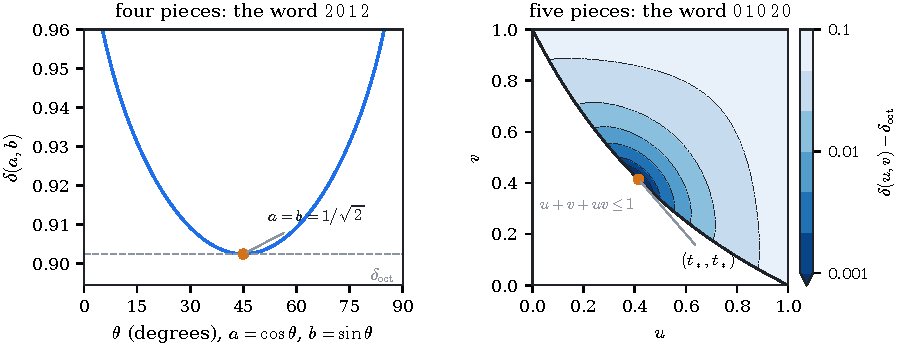
\includegraphics[width=\textwidth]{figures/fig-terminal-densities.pdf}
 \caption{Left: the four-piece density $\delta(\cos\theta,\sin\theta)$ of
 \eqref{eq:four-density}; its minimum $\doct$ is attained only at $\theta=45^\circ$, the octagon.
 Right: the excess $\delta(u,v)-\doct$ of the five-piece density \eqref{eq:five-density} over its
 domain $u,v\in(0,1)$, $u+v+uv>1$, on a logarithmic colour scale; it is positive everywhere and
 tends to $0$ only at the boundary point $(t_*,t_*)$, $t_*=\sqrt2-1$, where the middle factor
 tends to $1$. Both are computed from the cycle data; the script also checks the closure, the
 forced margins and the cost identity at random parameters.}
 \label{fig:terminal-densities}
\end{figure}

\begin{corollary}\label{cor:four-equality}
A closed vertex cycle with four pieces has raw cost at least $8\doct$. If its raw cost is
$8\doct$, then every factor is $\sqrt2$, every switch is forward, and its initial margins are
those of the octagon: the active margin $m_0(i_0)$ and the margin $m_0(i_0+2)$ equal
$2/\sqrt{2\sqrt2-1}$, and $m_0(i_0+1)=2(\sqrt2-1)/\sqrt{2\sqrt2-1}$.
\end{corollary}

\begin{proof}
Relabel to the word $2\,0\,1\,2$ and apply \cref{lem:four-param} and \cref{thm:four-density}. At
equality $a=b=1/\sqrt2$, so every factor is $\sqrt2$, $s=\sqrt2$, $\mathcal N=2\sqrt2-1$, and
\eqref{eq:four-margins} gives the stated margins.
\end{proof}

With active margin $a_k=2/\sqrt{2\sqrt2-1}$ and factor $\sqrt2$, each piece lasts
$(a_k/2)\log q_k=\log2/(2\sqrt{2\sqrt2-1})$, the octagon's switching time $\tsw$.

\subsection{Five pieces}\label{sec:terminal-five}

By \cref{prop:terminal-words}, a five-piece cycle that is not entirely reverse can be rebased
and relabeled to the word $0\,1\,0\,2\,0$, whose switches have the signs $+--++$. Its closure has
a two-parameter family of solutions. Put
\[
 P(t)=\frac{1+t^2}{2t},\qquad Q(t)=\frac{1+t^2}{1-t^2}\qquad(0<t<1).
\]

\begin{lemma}[Five-piece closure]\label{lem:five-closure}
If $p,q,r,s,z>1$ and
\[
 \widetilde T_0(p)\,\widetilde T_1(q)\,\widetilde T_0(r)\,\widetilde T_2(s)\,\widetilde T_0(z)
 =\widetilde R,
\]
then $p^2(q^2-1)=q^2$, $z^2(s^2-1)=s^2$ and $r^2=(q^2-1)(s^2-1)$. Consequently there are $u,v\in(0,1)$ with $u+v+uv>1$ and
\[
 (p,q,r,s,z)=\Bigl(P(u),\ Q(u),\ \frac{4uv}{(1-u^2)(1-v^2)},\ Q(v),\ P(v)\Bigr).
\]
\end{lemma}

\begin{proof}
The three relations come from the entries of the product compared with $\widetilde R$. Every
$q>1$ is $Q(u)$ for $u=\sqrt{(q-1)/(q+1)}\in(0,1)$, and then $p^2=q^2/(q^2-1)$ gives $p=P(u)$;
likewise for $s,z$ and $v$, and $r^2=(Q(u)^2-1)(Q(v)^2-1)$ gives the middle factor. Finally $r>1$
is equivalent to $u+v+uv>1$ by the factorization
$4uv-(1-u^2)(1-v^2)=(u+v+uv-1)(u+v+1-uv)$, whose second factor is positive.
\end{proof}

Put $d=(1-u)(1-v)$ and
\[
 F(t)=\Bigl(\frac{1+t}{1-t}\Bigr)^{2}\log\frac{1+t^2}{2t}+\frac{1}{t^2}\log\frac{1+t^2}{1-t^2}
 +\log\frac{2t}{1-t^2},
\]
and define the \emph{five-piece density}
\begin{equation}\label{eq:five-density}
 \delta(u,v)=\frac{2(d+2)-\tfrac{d}{2}\bigl(F(u)+F(v)\bigr)}{4-d}.
\end{equation}

\begin{lemma}[Five-piece cycles]\label{lem:five-param}
Let $c$ be a closed vertex cycle with word $0\,1\,0\,2\,0$. There are $u,v\in(0,1)$ with
$u+v+uv>1$ such that the factors are those of \cref{lem:five-closure}, the initial margins are
\[
 (m_0(0),m_0(1),m_0(2))=\frac{2}{\sqrt{d(4-d)}}\bigl((1+u)(1-v),\ d,\ (1-u)(1+v)\bigr),
\]
and the raw cost is $8\,\delta(u,v)$.
\end{lemma}

\begin{proof}
As for four pieces, the twist gives two linear equations for the initial margins, which the
quadric normalizes. With $A=(1+u)(1-v)$ and $B=(1-u)(1+v)$, the active margins of the five pieces
are $A$, $d/u$, $d$, $d/v$, $B$, times $2/\sqrt{d(4-d)}$. The algebraic part of the raw cost (all
but the terms $-a_k^2\log q_k$) adds up to $16\,d(d+2)/(d(4-d))$, and the logarithmic part is
\[
 -\frac{4}{d(4-d)}\Bigl(A^2\log P(u)+\frac{d^2}{u^2}\log Q(u)+d^2\log r+\frac{d^2}{v^2}\log Q(v)
 +B^2\log P(v)\Bigr).
\]
Since $A/d=(1+u)/(1-u)$, $B/d=(1+v)/(1-v)$ and
$\log r=\log\frac{2u}{1-u^2}+\log\frac{2v}{1-v^2}$, the bracket is $d^2(F(u)+F(v))$, and the
raw cost is $8\delta(u,v)$.
\end{proof}

\begin{theorem}[The five-piece density]\label{thm:five-density}
For $u,v\in(0,1)$ with $u+v+uv>1$, $\delta(u,v)>\doct$.
\end{theorem}

The proof is in \cref{app:five-density}; here is its structure. The function $F$ enters only
through $F(t)+2\log(1-t)$, and this function of one variable is at most its value at
$t_*=\sqrt2-1$, namely $(3+2\sqrt2)\log2+2\log(2-\sqrt2)$. Summing over
$t=u,v$ bounds $F(u)+F(v)$ above by a function of $d$ alone, hence $\delta(u,v)$ below by a
function of $d$. The constraint $u+v+uv>1$ gives $d<d_*=(2-\sqrt2)^2$, and at $d=d_*$ the lower
bound equals $\doct$ exactly. A tangent-line estimate for $d\log d$ at $d_*$ shows that the bound
exceeds $\doct$ for $d<d_*$. The infimum of $\delta(u,v)$ is approached only as $u,v\to t_*$,
where $d\to d_*$ and the middle factor $r$ tends to~$1$: the five-piece period degenerates into
the octagon's four pieces (right panel of \cref{fig:terminal-densities}).

\subsection{The terminal theorem}\label{sec:terminal-theorem}

\begin{theorem}[Terminal comparison]\label{thm:terminal}
Every normal vertex period with at most five pieces costs at least $\Aoct$.
\end{theorem}

\begin{proof}
Let $c$ be the cycle of the period (\cref{lem:term-cycle}). It is not entirely reverse, by
\cref{thm:class-R}, which holds for every number of pieces. By \cref{prop:terminal-words}, either
it has four pieces, and then its raw cost is at least $8\doct$ by \cref{cor:four-equality}, or it
has five pieces and is a rebasing and relabeling of a cycle with word $0\,1\,0\,2\,0$, whose raw
cost exceeds $8\doct$ by \cref{lem:five-param} and \cref{thm:five-density}. By
\cref{lem:term-cycle},
$\cost\ge\frac{\sqrt3}{4}\cdot8\doct=\sqrt{12}\,\doct=\Aoct$.
\end{proof}

No competitiveness and no compact domain are needed here. The equality case identifies the
trajectory itself.

\begin{proposition}[Terminal equality]\label{prop:terminal-equality}
Let $P$ be a normal vertex period with at most five pieces and cost $\Aoct$. Then $T=\tf$, and
there is $r\in\N$ such that, for $t\in[0,T]$,
\[
 R^{-r}g(t)R^{r}=g_{\mathrm{oct}}(t),\qquad R^{-r}X(t)R^{r}=X_{\mathrm{oct}}(t),
\]
where $(g_{\mathrm{oct}},X_{\mathrm{oct}})$ is the trajectory of the smoothed octagon
(\cref{prop:octagon-trajectory}).
\end{proposition}

\begin{proof}
A five-piece cycle that is not entirely reverse has raw cost strictly above $8\doct$, and the
entirely reverse case is excluded by \cref{thm:class-R}, so $N=4$. By \cref{cor:four-equality} the period has four forward pieces,
all factors $\sqrt2$, and the octagon's initial margins. A traceless matrix is determined by its
margins, so after relabeling by a power of $R$ the initial state is $\Phi(0,y_0)$ with
$y_0^2=(2\sqrt2-1)/3$, and the control agrees almost everywhere with the octagon's control
$\ee_2\ee_0\ee_1\ee_2$ on four pieces of length $\tsw$. Changing a control on a null set does not
change a Carath\'eodory solution, and the octagon's trajectory is the unique solution with
$g(0)=I$ and $X(0)=\Phi(0,y_0)$, by uniqueness of solutions of the state equations with a fixed
vertex control on each piece.
\end{proof}

\subsection{Proofs of the lower bounds}\label{sec:terminal-proofs}

The chain of reductions now closes. Recall that a global minimizer is an admissible trajectory
whose cost is at most that of every admissible trajectory (\cref{def:global-minimizer}).

\begin{theorem}[Cost of a minimizer]\label{thm:minimizer-cost}
Every global minimizer of the control problem costs at least $\Aoct$.
\end{theorem}

\begin{proof}
Let $(T,u,g,X)$ be a global minimizer. The octagon's trajectory is admissible and costs $\Aoct$
(\cref{prop:octagon-trajectory}), so $\cost(T,X)\le\Aoct$: the minimizer is competitive. By
\cref{thm:finite-normal}, rebased at a
switch it is a normal vertex period $P$ with the same terminal time and cost, whose state stays
in $\hstarstar$. By \cref{thm:at-most-five}, $P$ has at most five pieces, and by
\cref{thm:terminal}, $\cost(P)\ge\Aoct$.
\end{proof}

\begin{proof}[Proof of \cref{thm:control}]
Let $(T,u,g,X)$ be admissible, with any terminal time and any measurable control. By
\cref{thm:equivalence} a global minimizer $(T',u',g',X')$ exists: the realization of a worst disk.
By \cref{thm:minimizer-cost} and minimality, $\Aoct\le\cost(T',X')\le\cost(T,X)$, and
$\Aoct=\sqrt{12}\,\doct$.
\end{proof}

\begin{proof}[Proof of \cref{thm:main}\textup{(b)}]
By \cref{thm:equivalence} there is a worst disk $K_0$, a convex disk symmetric about the origin
whose greatest packing density is the least among all such disks, and its realization is a global
minimizer of cost $\sqrt{12}\,\delta(K_0)$. By \cref{thm:minimizer-cost},
$\sqrt{12}\,\delta(K_0)\ge\Aoct$, that is, $\delta(K_0)\ge\doct$. Now let $K$ be a convex disk with
a centre $c$, so that $2c-x\in K$ for $x\in K$. Its translate $K-c$ is a convex disk symmetric
about the origin, and translation does not change the greatest packing density, since a translate
is a congruent copy (\cref{prop:converse}). Hence $\delta(K)=\delta(K-c)\ge\delta(K_0)\ge\doct$.
\end{proof}
